\documentclass[
11pt, % The default document font size, options: 10pt, 11pt, 12pt
codirector, % Uncomment to add a codirector to the title page
]{charter} 


% El títulos de la memoria, se usa en la carátula y se puede usar el cualquier lugar del documento con el comando \ttitle
\titulo{Predicción de eventos climáticos y meteorológicos extremos utilizando inteligencia artificial} 

% Nombre del posgrado, se usa en la carátula y se puede usar el cualquier lugar del documento con el comando \degreename
%\posgrado{Carrera de Especialización en Sistemas Embebidos} 
%\posgrado{Carrera de Especialización en Internet de las Cosas} 
\posgrado{Carrera de Especialización en Inteligencia Artificial}
%\posgrado{Maestría en Sistemas Embebidos} 
%\posgrado{Maestría en Internet de las cosas}
% IMPORTANTE: no omitir titulaciones ni tildación en los nombres, también se recomienda escribir los nombres completos (tal cual los tienen en su documento)
% Tu nombre, se puede usar el cualquier lugar del documento con el comando \authorname
\autor{Ing. Sevann Radhak Triztan}

% El nombre del director y co-director, se puede usar el cualquier lugar del documento con el comando \supname y \cosupname y \pertesupname y \pertecosupname
\director{Título y Nombre del director}
\pertenenciaDirector{pertenencia} 
\codirector{Título y Nombre del codirector} % para que aparezca en la portada se debe descomentar la opción codirector en los parámetros de documentclass
\pertenenciaCoDirector{FIUBA}

% Nombre del cliente, quien va a aprobar los resultados del proyecto, se puede usar con el comando \clientename y \empclientename

\cliente{Lic. Carlos Roberto Salinas}
\empresaCliente{Dirección de Meteorología e Hidrología}
 
\fechaINICIO{18 de junio de 2024}		%Fecha de inicio de la cursada de GdP \fechaInicioName
\fechaFINALPlan{13 de agosto de 2024} 	%Fecha de final de cursada de GdP
\fechaFINALTrabajo{en el mes de diciembre de 2024}	%Fecha de defensa pública del trabajo final

\begin{document}

\maketitle
\thispagestyle{empty}
\pagebreak


\thispagestyle{empty}
{\setlength{\parskip}{0pt}
\tableofcontents{}
}
\pagebreak


\section*{Registros de cambios}
\label{sec:registro}


\begin{table}[ht]
\label{tab:registro}
\centering
\begin{tabularx}{\linewidth}{@{}|c|X|c|@{}}
\hline
\rowcolor[HTML]{C0C0C0} 
Revisión & \multicolumn{1}{c|}{\cellcolor[HTML]{C0C0C0}Detalles de los cambios realizados} & Fecha      \\ \hline
0      & Creación del documento                                 &\fechaInicioName \\ \hline
1      & Se completa hasta el punto 5 inclusive                & 2 de julio de 2024 \\ \hline
2      & Se completa hasta el punto 9 inclusive				 & 9 de julio de 2024 \\ \hline
3      & Se completa hasta el punto 12 inclusive				 & 26 de julio de 2024 \\ \hline
3      & Se completa hasta el punto 15 inclusive				 & 29 de julio de 2024 \\ \hline
%		  Se puede agregar algo más \newline
%		  En distintas líneas \newline
%		  Así                                                    & {día} de {mes} de 202X \\ \hline
%3      & Se completa hasta el punto 12 inclusive                & {día} de {mes} de 202X \\ \hline
%4      & Se completa el plan	                                 & {día} de {mes} de 202X \\ \hline

% Si hay más correcciones pasada la versión 4 también se deben especificar acá

\end{tabularx}
\end{table}

\pagebreak



\section*{Acta de constitución del proyecto}
\label{sec:acta}

\begin{flushright}
Buenos Aires, \fechaInicioName
\end{flushright}

\vspace{2cm}

Por medio de la presente se acuerda con el \authorname\hspace{1px} que su Trabajo Final de la \degreename\hspace{1px} se titulará ``\ttitle'' y consistirá esencialmente en la implementación de técnicas de inteligencia artificial (IA) para mejorar las predicciones de eventos climáticos y meteorológicos extremos. El trabajo tendrá un presupuesto preliminar estimado de 600 horas y un costo estimado de USD \$ 16,800, con fecha de inicio el \fechaInicioName\hspace{1px} y fecha de presentación pública \fechaFinalName.

Se adjunta a esta acta la planificación inicial.

\vfill

% Esta parte se construye sola con la información que hayan cargado en el preámbulo del documento y no debe modificarla
\begin{table}[ht]
\centering
\begin{tabular}{ccc}
\begin{tabular}[c]{@{}c@{}}Dr. Ing. Ariel Lutenberg \\ Director posgrado FIUBA\end{tabular} & \hspace{2cm} & \begin{tabular}[c]{@{}c@{}}\clientename \\ \empclientename \\ Cliente \end{tabular} \vspace{2.5cm} \\ 
\multicolumn{3}{c}{\begin{tabular}[c]{@{}c@{}} \supname \\ Director del Trabajo Final\end{tabular}} \vspace{2.5cm} \\
\end{tabular}
\end{table}


\section{1. Descripción técnica-conceptual del proyecto a realizar}
\label{sec:descripcion}

El cambio climático y los eventos meteorológicos extremos presentan desafíos críticos a nivel global y local, afectando la vida, la infraestructura y la economía. En Paraguay, los eventos extremos como olas de calor, sequías y precipitaciones intensas han aumentado, destacando la necesidad urgente de mejorar la precisión y la efectividad de los pronósticos meteorológicos. 

Las actuales técnicas de monitoreo y predicción no siempre resultan suficientes para emitir advertencias tempranas y precisas. Este proyecto enfrenta el reto de adquirir, analizar y aplicar conocimientos para resolver problemas climatológicos complejos y busca utilizar la inteligencia artificial (IA) para analizar grandes volúmenes de datos meteorológicos y climáticos, tanto actuales como históricos, con el fin de mejorar la precisión de las predicciones y la toma de decisiones.

Este proyecto, propuesto por la \empclientename\hspace{1px} (DINAC) y el Parque Tecnológico Itaipu de Paraguay, busca abordar los desafíos actuales en la predicción de eventos climáticos extremos mediante el uso de herramientas de IA, contribuyendo así a mitigar los impactos del cambio climático en Paraguay y la región.

En la figura \ref{fig:diagBloques} se presenta el diagrama en bloques del sistema. Se observan los pasos propuestos para el desarrollo del presente proyecto. 

\begin{figure}[htpb]
\centering 
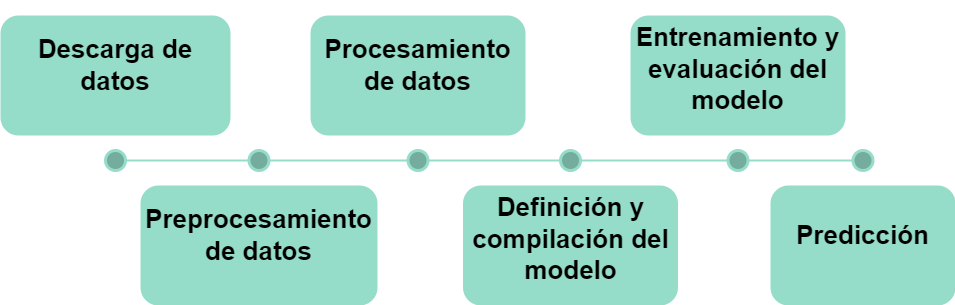
\includegraphics[width=.65\textwidth]{./Figuras/diagBloques.png}
\caption{Diagrama en bloques del sistema.}
\label{fig:diagBloques}
\end{figure}

\textbf{Descarga de datos:}
la \empclientename\hspace{1px} pondrá a disposición una base de datos para la obtención de datos históricos y actuales de las condiciones meteorológicas.

\textbf{Preprocesamiento de datos:}
se llevará a cabo un análisis de datos en crudo con el objetivo de dar tratamiento a datos vacíos, inconsistentes o conflictivos.

\textbf{Procesamiento de datos:}
serán aplicadas técnicas como la imputación de valores faltantes, reducción de dimensionalidad, estimación e interpretación de valores representativos, entre otras.

\textbf{Definición y compilación del modelo:}
diferentes modelos y técnicas serán propuestas, entrenadas y evaluadas para determinar el mejor modelo a utilizar.

\textbf{Entrenamiento y evaluación del modelo:}
el modelo seleccionado será entrenado con los datos procesados y evaluado aplicando técnicas avanzadas y métricas específicas para determinar su precisión y robustez.

\textbf{Predicción:}
una vez evaluado y ajustado el modelo, se procederá a realizar predicciones sobre los datos meteorológicos futuros, proporcionando información crítica para la toma de decisiones en la gestión de eventos climáticos extremos.


\vspace{25px}

\section{2. Identificación y análisis de los interesados}
\label{sec:interesados}

\begin{table}[ht]
%\caption{Identificación de los interesados}
%\label{tab:interesados}
\begin{tabularx}{\linewidth}{@{}|l|X|X|l|@{}}
\hline
\rowcolor[HTML]{C0C0C0} 
Rol           & Nombre y Apellido & Organización 	& Puesto 	\\ \hline
Cliente       & \clientename      &\empclientename	&   Gerente de Climatología     	\\ \hline
Product Owner       & \clientename      &\empclientename	&   Gerente de Climatología     	\\ \hline
Responsable   & \authorname       & FIUBA        	& Alumno 	\\ \hline
Orientador    & \supname	      & \pertesupname 	& Director del Trabajo Final \\ \hline
Usuario final & Dr. Sidney da Silva Viana                  & Central Hidroeléctrica Itaipu             	& Gerente de tecnologías en SI        	\\ \hline
\end{tabularx}
\end{table}

\begin{itemize}
	\item Cliente: el Dr. Ing. Sidney da Silva Vianna es experto en la temática, ejerce como Gerente de tecnologías en Sistemas de la Información (SI) y va a ayudar con la definición de los requerimientos y el desarrollo de la solución.
	\item Usuario final: Lic. Carlos Roberto Salinas, ejerce como 	Gerente de Climatología en la Dirección de Meteorología e Hidrología y la Dirección Nacional de Aeronáutica Civil. Proporcionará información útil respecto a las expectativas reales del usuario.
\end{itemize}

\section{3. Propósito del proyecto}
\label{sec:proposito}

Desarrollar un sistema de predicción de eventos climáticos y meteorológicos extremos utilizando técnicas de IA. Este sistema tiene como objetivo principal mejorar la precisión y la rapidez de los pronósticos meteorológicos, facilitando respuestas más efectivas ante los fenómenos climáticos adversos y contribuyendo a la mitigación de sus impactos en Paraguay y sus alrededores.

\section{4. Alcance del proyecto}
\label{sec:alcance}

El proyecto incluye:
\begin{itemize}
	\item Recolección y preprocesamiento de datos:
		\begin{itemize}
		\item Obtención de datos meteorológicos históricos y actuales almacenados en la base de
datos de la DINAC.
		\item Filtrado, normalización y preprocesamiento de los datos para su uso en los modelos de IA.
		\end{itemize}
	\item Investigación y desarrollo de modelos de IA:
		\begin{itemize}
		\item Identificación y selección de modelos de IA adecuados para el análisis de datos meteorológicos.
		\item Desarrollo y ajuste de modelos de IA para predicción climática a corto y largo plazo.
		\end{itemize}
	\item Implementación de la plataforma de predicción:
		\begin{itemize}
		\item Diseño y desarrollo de una plataforma tecnológica que integre el modelo de IA desarrollado.
		\item Implementación de interfaces de usuario para la visualización de predicciones y alertas.
		\end{itemize}
	\item Validación y optimización de modelos:
		\begin{itemize}
		\item Pruebas y validación de los modelos de predicción utilizando datos históricos y actuales.
		\item Optimización continua de los modelos para mejorar su precisión y eficiencia.
		\end{itemize}
	\item Gestión y monitoreo del proyecto:
		\begin{itemize}
		\item Establecimiento de un cronograma detallado y seguimiento del progreso del proyecto.
		\item Gestión de riesgos y resolución de problemas durante el desarrollo del proyecto.
		\end{itemize}
	
\end{itemize}

El proyecto no incluye:
\begin{itemize}
	\item Implementación de infraestructura física:
		\begin{itemize}
		\item La construcción, instalación o conexión a estaciones meteorológicas no está incluida.
		\item La actualización o mejora de la infraestructura física existente de recopilación de datos meteorológicos no forma parte del alcance del proyecto.
		\end{itemize}
	\item Mantenimiento a largo plazo:
		\begin{itemize}
		\item El mantenimiento continuo de la plataforma y los sistemas desarrollados, después de la finalización del proyecto, no está incluido.
		\item Las tareas de mantenimiento o soporte post-implementación.
		\end{itemize}
	\item Distribución y gestión de alertas:
		\begin{itemize}
		\item La implementación de sistemas de distribución masiva de alertas no está incluida.
		\end{itemize}
	\item Integración con sistemas externos:
		\begin{itemize}
		\item La integración completa con otros sistemas de gestión de emergencias o bases de datos externas fuera del ámbito meteorológico no se incluye.
		\item La integración directa con sistemas externos.
		\end{itemize}

\end{itemize}

\section{5. Supuestos del proyecto}
\label{sec:supuestos}

Para el desarrollo del presente proyecto se supone que: 

\begin{itemize}
	\item Se tendrá acceso continuo a una fuente de datos provista por la DINAC.
	\item La DINAC cuenta con una infraestructura tecnológica adecuada que permitirá el correcto entrenamiento y despliegue de la solución.
	\item Se fijarán y desarrollarán reuniones periódicas con el cliente para abordar temas relacionados con el proyecto.
	\item Se mantendrá la relación mediante el programa de vinculación con la DINAC hasta finalizar el desarrollo del proyecto.
	\item Se contará con la colaboración de expertos: se asume que será posible obtener la colaboración de expertos en el área que se requiera, desde las cuestiones climatológicas hasta las que involucren técnicas de inteligencia artificial.
\end{itemize}

\section{6. Requerimientos}
\label{sec:requerimientos}

\begin{enumerate}
	\item Requerimientos funcionales:
		\begin{enumerate}
			\item El sistema debe ser capaz de recolectar datos meteorológicos históricos y actuales de la base de datos de la DINAC.
			\item El sistema debe implementar y entrenar múltiples modelos de IA para determinar su conveniencia en términos de precisión, eficiencia y robustez.
			\item El sistema debe superar a los modelos actuales en términos de precisión.
			\item El sistema debe emitir advertencias tempranas basadas en las predicciones de eventos extremos.
		\end{enumerate}
	\item Requerimientos no funcionales:
		\begin {enumerate}
			\item La solución debe estar programada de forma modular para que el código de sus características funcionales pueda ser fácilmente reutilizado y/o escalado.
			\item El sistema debe ser capaz de procesar grandes volúmenes de datos sin degradar su rendimiento.
		\end{enumerate}
	\item Requerimientos de datos:
		\begin {enumerate}
			\item Los datos meteorológicos históricos y actuales deben estar disponibles en la base de datos de la DINAC.
			\item Deben definirse formatos estándar para la importación y exportación de datos.
		\end{enumerate}
	\item Requerimientos de documentación:
		\begin{enumerate}
			\item Debe crearse una documentación técnica del sistema, incluyendo su arquitectura, diseño y funcionamiento.
		\end{enumerate}
	\item Requerimientos de testing:
		\begin{enumerate}
			\item La efectividad de los modelos será acordada y evaluada en conjunto con el cliente.
		\end{enumerate}
\end{enumerate}

\section{7. Historias de usuarios (\textit{Product backlog})}
\label{sec:backlog}

Las historias están valoradas en un sistema de puntaje (\textit{story points}) basado en la estimación de tres categorías: dificultad, complejidad e incertidumbre del trabajo en cada una. La escala de \textit{story points} es:

\begin{itemize}
\item Trivial: 1
\item Bajo: 2
\item Medio: 3
\item Alto: 5 o más
\end{itemize}

\begin{enumerate}
\item Como Product Owner, quiero obtener datos meteorológicos históricos y actuales de la base de datos de la DINAC para realizar análisis precisos.

\textit{Story points}: 8 (complejidad: 1, dificultad: 2, incertidumbre: 5)

\item Como Product Owner, quiero limpiar y normalizar los datos meteorológicos para garantizar su calidad ante los modelos de IA que serán entrenados.

\textit{Story points}: 13 (complejidad: 5, dificultad: 5, incertidumbre: 3)

\item Como Product Owner, quiero aplicar técnicas de imputación de valores faltantes para manejar datos incompletos.

\textit{Story points}: 8 (complejidad: 3, dificultad: 3, incertidumbre: 2)

\item Como Product Owner, quiero utilizar modelos de IA para predecir eventos climáticos extremos y mejorar la precisión de las predicciones.

\textit{Story points}: 13 (complejidad: 5, dificultad: 5, incertidumbre: 3)

\item Como Usuario, quiero comparar los resultados obtenidos de los modelos de IA entrenados con el modelo actual para seleccionar el más adecuado para nuestras necesidades.

\textit{Story points}: 13 (complejidad: 5, dificultad: 3, incertidumbre: 5)

\item Como Product Owner, quiero emitir alertas tempranas de eventos climáticos extremos para tomar decisiones informadas y mitigar impactos.

\textit{Story points}: 13 (complejidad: 3, dificultad: 5, incertidumbre: 5)

\item Como Product Owner, quiero elaborar una publicación científica basada en los resultados obtenidos del proyecto para contribuir al conocimiento en el campo de la predicción de eventos climáticos extremos.

\textit{Story points}: 8 (complejidad: 2, dificultad: 3, incertidumbre: 3)
\end{enumerate}

\section{8. Entregables principales del proyecto}
\label{sec:entregables}

\begin{itemize}
	\item Documento de especificación de requerimientos.
	\item Modelos de IA entrenados y evaluados.
	\item Sistema de predicción implementado.
	\item Informe final del proyecto.
	\item Código fuente y recursos digitales.
	\item Memoria del trabajo final.
	\item Publicación científica basada en los resultados del proyecto.
\end{itemize}

\section{9. Desglose del trabajo en tareas}
\label{sec
}

\begin{enumerate}
\item Grupo de tareas 1: recolección y preprocesamiento de datos (100 h)
	\begin{enumerate}
	\item Tarea 1: definir y establecer la conexión con la base de datos de la DINAC (20 h).
	\item Tarea 2: desarrollar scripts para la extracción automática de datos históricos y actuales (10 h).
	\item Tarea 3: validar la integridad y calidad de los datos recolectados (10 h).
	\item Tarea 4: limpieza y normalización de datos para eliminar valores atípicos y errores (25 h).
	\item Tarea 5: aplicación de técnicas de imputación para manejar datos faltantes (30 h).
	\item Tarea 6: documentar el proceso de obtención de datos (5 h)
	\end{enumerate}
\item Grupo de tareas 2: desarrollo y evaluación de modelos de IA (180 h)
	\begin{enumerate}
	\item Tarea 7: investigar y seleccionar modelos apropiados para el análisis de datos meteorológicos (30 h).
	\item Tarea 8: implementar los modelos seleccionados en el entorno de desarrollo (50 h).
	\begin{enumerate}
	\item Subtarea 8.1: configurar el entorno de desarrollo para la implementación de modelos (10 h).	
	\item Subtarea 8.2: desarrollar el código base para el primer modelo de IA (20 h).
	\item Subtarea 8.3: desarrollar el código base para el segundo modelo de IA (20 h).
	\end{enumerate}		
	\item Tarea 9: entrenar y ajustar los modelos con datos preprocesados (60 h).
	\begin{enumerate}
	\item Subtarea 9.1: entrenar el primer modelo de IA con los datos preprocesados (20 h).
	\item Subtarea 9.2: entrenar el segundo modelo de IA con los datos preprocesados (20 h).
	\item Subtarea 9.3: realizar ajustes y optimizaciones en el primer modelo (10 h).
	\item Subtarea 9.4: realizar ajustes y optimizaciones en el segundo modelo (10 h).
	\end{enumerate}	
	\item Tarea 10: comparar la precisión y eficiencia de los modelos implementados con el modelo actual (40 h).
	\begin{enumerate}
	\item Subtarea 10.1: definir métricas y criterios de evaluación para los modelos (10 h).
	\item Subtarea 10.2: realizar pruebas de precisión y eficiencia en el primer modelo (15 h).
	\item Subtarea 10.3: realizar pruebas de precisión y eficiencia en el segundo modelo (15 h).
	\end{enumerate}
	\end{enumerate}
\item Grupo de tareas 3: implementación del sistema y documentación (150 h).
\begin{enumerate}
	\item Tarea 11: diseñar la arquitectura del sistema de predicción de eventos climáticos (40 h).
	\item Tarea 12: implementar el sistema de predicción de eventos climáticos (40 h).
	\item Tarea 13: implementar el proceso de emisión de predicciones y alertas (30 h).
	\item Tarea 14: realizar pruebas de aceptación con el cliente para validar la funcionalidad del sistema (20 h).
	\item Tarea 15: elaborar la documentación técnica del sistema y los manuales de usuario (20 h).
	\end{enumerate}
\item Grupo de tareas 4: gestión del proyecto y presentación (50 h).
\begin{enumerate}
	\item Tarea 16: gestionar riesgos y problemas durante el desarrollo del proyecto (30 h).
	\item Tarea 17: preparar la presentación pública del proyecto y demostración ante el jurado (20 h).
	\end{enumerate}
\item Grupo de tareas 5: elaboración de una publicación científica (60 h).
\begin{enumerate}
	\item Tarea 24: investigación y recopilación de información relevante (10 h).
	\item Tarea 25: redacción del artículo científico (30 h).
	\item Tarea 26: revisión y corrección del artículo científico (20 h).
	\end{enumerate}		
\item Grupo de tareas 6: generación de entregables y proceso de cierre (60 h).
\begin{enumerate}
	\item Tarea 18: inicio de la elaboración de la memoria técnica (20 h).
	\item Tarea 19: revisión y correcciones de la memoria técnica (5 h).
	\item Tarea 20: finalización de la elaboración de la memoria técnica (20 h).
	\item Tarea 21: revisión y correcciones de la memoria técnica final (5 h).
	\item Tarea 22: elaboración de la presentación final (8 h).
	\item Tarea 23: revisión y correcciones de la presentación final (2 h).
	\end{enumerate}
\end{enumerate}

Cantidad total de horas: 600 h.

\section{10. Diagrama de Activity On Node}
\label{sec:AoN}

En la figura \ref{fig:AoN} se observa el diagrama de \textit{Activity on Node} del proyecto. Las actividades relacionadas con el camino crítrico, señaladas con flechas negras, implican 545 horas de trabajo.

\begin{figure}[htpb]
\centering 
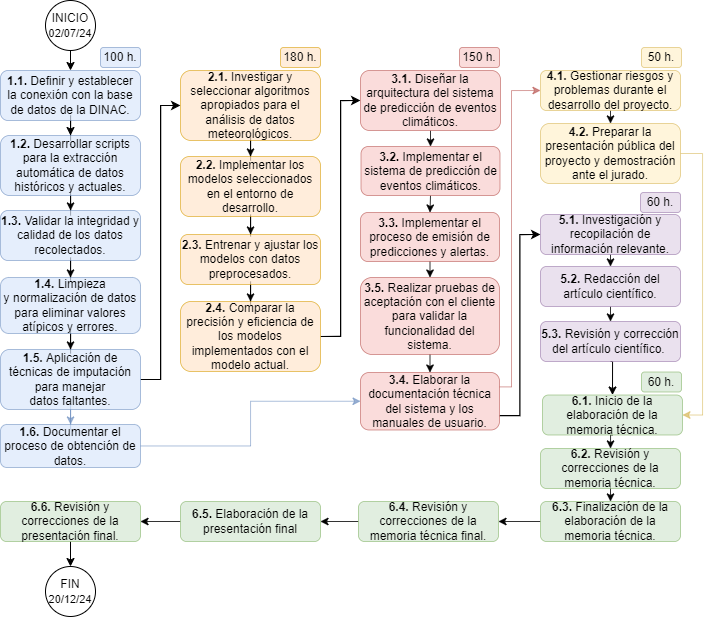
\includegraphics[width=.8\textwidth]{./Figuras/AoN.png}
\caption{Diagrama de \textit{Activity on Node}.}
\label{fig:AoN}
\end{figure}

\section{11. Diagrama de Gantt}
\label{sec:gantt}

En la figura \ref{fig:ganttchart} se observa el diagrama de \textit{Gantt} del proyecto.

\begin{landscape}
\centering 

\begin{figure}[htpb]
  \begin{center}
    \begin{ganttchart}[
      time slot unit=day,
      time slot format=isodate,
      x unit=0.09cm,
      y unit title=0.5cm,
      y unit chart=0.4cm,
      milestone/.append style={xscale=4},
      vgrid,
      hgrid,
      bar/.append style={fill=blue!50},
      bar label font=\tiny,
      group/.append style={fill=blue!20},
      group label font=\tiny,
      bar height=0.6
      ]{2024-06-01}{2024-12-31}
      
      % Títulos
      \gantttitlecalendar*{2024-06-01}{2024-12-31}{year} \\
      \gantttitlecalendar*{2024-06-01}{2024-12-31}{month} \\
      
      % Grupo de tareas 1: Recolección y preprocesamiento de datos
      \ganttgroup{1: Recolección y preprocesamiento de datos}{2024-08-01}{2024-09-15} \\
      \ganttbar[name=T1]{1.1: Definir y establecer conexión}{2024-08-01}{2024-08-07} \\
      \ganttbar[name=T2]{1.2: Desarrollar scripts de extracción}{2024-08-08}{2024-08-14} \\
      \ganttbar[name=T3]{1.3: Validar integridad y calidad de datos}{2024-08-15}{2024-08-21} \\
      \ganttbar[name=T4]{1.4: Limpieza y normalización de datos}{2024-08-22}{2024-09-02} \\
      \ganttbar[name=T5]{1.5: Aplicación de técnicas de imputación}{2024-09-03}{2024-09-15} \\
      \ganttbar[name=T6]{1.6: Documentar proceso de obtención (en paralelo)}{2024-08-01}{2024-09-15} \\
      
      % Grupo de tareas 2: Desarrollo y evaluación de modelos de IA
      \ganttgroup{2: Desarrollo y evaluación de modelos de IA}{2024-09-16}{2024-10-31} \\
      \ganttbar[name=T7]{2.1: Investigar y seleccionar modelos}{2024-09-16}{2024-09-30} \\
      \ganttbar[name=T8]{2.2: Implementar modelos seleccionados}{2024-10-01}{2024-10-15} \\
      \ganttbar[name=T9]{2.3: Entrenar y ajustar modelos}{2024-10-16}{2024-10-31} \\
      \ganttbar[name=T10]{2.4: Comparar precisión y eficiencia}{2024-10-31}{2024-10-31} \\
      
      % Grupo de tareas 3: Implementación del sistema y documentación
      \ganttgroup{3: Implementación del sistema y documentación}{2024-10-16}{2024-11-30} \\
      \ganttbar[name=T11]{3.1: Diseñar la arquitectura del sistema}{2024-10-16}{2024-10-31} \\
      \ganttbar[name=T12]{3.2: Implementar proceso de predicciones y alertas}{2024-11-01}{2024-11-10} \\
      \ganttbar[name=T13]{3.3: Integrar modelos de IA con la plataforma}{2024-11-11}{2024-11-20} \\
      \ganttbar[name=T14]{3.4: Realizar pruebas de aceptación con el cliente}{2024-11-21}{2024-11-26} \\
      \ganttbar[name=T15]{3.5: Elaborar documentación técnica}{2024-11-27}{2024-11-30} \\
      
      % Grupo de tareas 4: Gestión del proyecto y presentación
      \ganttgroup{4: Gestión del proyecto y presentación}{2024-06-01}{2024-12-31} \\
      \ganttbar[name=T16]{4.1: Gestionar riesgos y problemas}{2024-06-01}{2024-12-01} \\
      \ganttbar[name=T17]{4.2: Preparar la presentación pública}{2024-12-02}{2024-12-31} \\
      
      % Grupo de tareas 5: Generación de entregables y proceso de cierre
      \ganttgroup{5: Generación de entregables y proceso de cierre}{2024-12-01}{2024-12-31} \\
      \ganttbar[name=T18]{5.1: Inicio elaboración memoria técnica}{2024-12-01}{2024-12-10} \\
      \ganttbar[name=T19]{5.2: Revisión y correcciones de la memoria}{2024-12-11}{2024-12-15} \\
      \ganttbar[name=T20]{5.3: Fin de elaboración memoria técnica}{2024-12-16}{2024-12-22} \\
      \ganttbar[name=T21]{5.4: Revisión y correcciones de la memoria}{2024-12-23}{2024-12-27} \\
      \ganttbar[name=T22]{5.5: Elaboración de la presentación final}{2024-12-28}{2024-12-30} \\
      \ganttmilestone[name=M1]{5.6: Ensayo de la presentación}{2024-12-31} \\
      
      % Elaboración de publicación científica
      \ganttgroup{6: Elaboración de publicación científica}{2024-12-01}{2024-12-31} \\
      \ganttbar[name=T23]{6.1: Elaboración de la publicación científica}{2024-12-01}{2024-12-31} \\
    \end{ganttchart}
  \end{center}
  \caption{Diagrama de Gantt}
  \label{fig:ganttchart}
\end{figure}

\end{landscape}

\section{12. Presupuesto detallado del proyecto}
\label{sec:presupuesto}

\begin{table}[htpb]
\centering
\begin{tabularx}{\linewidth}{@{}|X|c|r|r|@{}}
\hline
\rowcolor[HTML]{C0C0C0} 
\multicolumn{4}{|c|}{\cellcolor[HTML]{C0C0C0}COSTOS DIRECTOS} \\ \hline
\rowcolor[HTML]{C0C0C0} 
Descripción &
  \multicolumn{1}{c|}{\cellcolor[HTML]{C0C0C0}Cantidad} &
  \multicolumn{1}{c|}{\cellcolor[HTML]{C0C0C0}Valor unitario} &
  \multicolumn{1}{c|}{\cellcolor[HTML]{C0C0C0}Valor total} \\ \hline
Hora de investigación y desarrollo &
  600 h &
  \$20 USD &
  \$12000 USD \\ \hline
Google Colaboratory &
  330 h &
  \$0 USD &
  \$0 USD \\ \hline
 &
  \multicolumn{1}{c|}{} &
  \multicolumn{1}{c|}{} &
  \multicolumn{1}{c|}{} \\ \hline
\multicolumn{3}{|c|}{SUBTOTAL} &
  \$12000 USD \\ \hline
\rowcolor[HTML]{C0C0C0} 
\multicolumn{4}{|c|}{\cellcolor[HTML]{C0C0C0}COSTOS INDIRECTOS} \\ \hline
\rowcolor[HTML]{C0C0C0} 
Descripción &
  \multicolumn{1}{c|}{\cellcolor[HTML]{C0C0C0}Cantidad} &
  \multicolumn{1}{c|}{\cellcolor[HTML]{C0C0C0}Valor unitario} &
  \multicolumn{1}{c|}{\cellcolor[HTML]{C0C0C0}Valor total} \\ \hline
Notebook &
  1 unidad &
  \$1200 USD &
  \$1200 USD \\ \hline
Imprevistos y contingencias (30\% de costos directos) &
  - &
  - &
  \$3600 USD \\ \hline
\multicolumn{3}{|c|}{SUBTOTAL} &
  \$4800 USD \\ \hline
\rowcolor[HTML]{C0C0C0}
\multicolumn{3}{|c|}{TOTAL} &
  \$16800 USD \\ \hline
\end{tabularx}%
\end{table}

La tasa de cambio oficial vigente a la fecha, 26 de julio de 2024, es de USD \$1 = ARS \$ 928.11. Por tal motivo, se ha calculado que el valor total de USD \$ 16.800 equivale a ARS \$15'606.042. 

\section{13. Gestión de riesgos}
\label{sec:riesgos}

\subsection{Identificación de riesgos y estimación de consecuencias}

Se utilizará una escala de 1 a 10 para cuantificar la severidad (S) y la ocurrencia (O), siendo 10 el valor máximo de probabilidad para ambas. Se identifican los siguientes riesgos para este proyecto.

\textbf{Riesgo 1: bajo desempeño de los modelos de IA.}
\begin{itemize}
  \item \textbf{Descripción:} los resultados obtenidos por los modelos están por debajo de los esperados, o su tiempo de procesamiento es mayor al esperado.
  \item \textbf{Severidad (S):} 10
  
  \textbf{Justificación:} si el desempeño de los modelos de IA no cumple con las expectativas de precisión, la utilidad del sistema se verá comprometida. Además, un tiempo de procesamiento excesivo puede impedir la detección y respuesta en tiempo real, afectando la capacidad del sistema para emitir alertas tempranas.
  \item \textbf{Probabilidad de ocurrencia (O):} 4
  
  \textbf{Justificación:} aunque los modelos puedan ser probados en otros contextos y demuestren resultados aceptables, la aplicación específica para la predicción de eventos climáticos extremos es novedosa y puede presentar desafíos imprevistos.
\end{itemize}

\textbf{Riesgo 2: interrupción en el acceso a los datos de la DINAC.}

\begin{itemize}
  \item \textbf{Descripción:} la disponibilidad continua de datos meteorológicos desde la base de datos de la DINAC es crucial para el desarrollo y funcionamiento del sistema.
  \item \textbf{Severidad (S):} 9
  
  \textbf{Justificación:} la falta de acceso a los datos impedirá la recolección y actualización de información necesaria para entrenar y validar los modelos, comprometiendo la precisión y actualidad de las predicciones.
  \item \textbf{Probabilidad de ocurrencia (O):} 3
  
  \textbf{Justificación:} aunque se asume que la DINAC proporcionará acceso continuo a los datos, existen factores externos que podrían afectar la disponibilidad, como problemas técnicos o administrativos.
\end{itemize}

\textbf{Riesgo 3: colaboración insuficiente de expertos.}

\begin{itemize}
  \item \textbf{Descripción:} la colaboración de expertos en climatología e inteligencia artificial es esencial para guiar el desarrollo del proyecto y validar los resultados obtenidos.
  \item \textbf{Severidad (S):} 8
  
  \textbf{Justificación:} la falta de orientación y validación por parte de expertos puede resultar en un desarrollo que no alcance los resultados óptimos en términos de precisión, lo que afectará la calidad del proyecto.
  \item \textbf{Probabilidad de ocurrencia (O):} 3
  
  \textbf{Justificación:} aunque se ha planeado obtener la colaboración de expertos, siempre existe la posibilidad de que estos no estén disponibles en los momentos necesarios debido a otros compromisos o falta de interés.
\end{itemize}

\textbf{Riesgo 4: problemas con la infraestructura tecnológica.}

\begin{itemize}
  \item \textbf{Descripción:} la infraestructura tecnológica de la DINAC debe ser adecuada para el correcto entrenamiento y despliegue de los modelos de IA.
  \item \textbf{Severidad (S):} 7
  
  \textbf{Justificación:} una infraestructura inadecuada puede limitar la capacidad de procesamiento de datos y el entrenamiento de modelos complejos, afectando el rendimiento y la efectividad del sistema.
  \item \textbf{Probabilidad de ocurrencia (O):} 4
  
  \textbf{Justificación:} aunque se asume que la DINAC cuenta con la infraestructura necesaria, existe la posibilidad de encontrar limitaciones técnicas no anticipadas durante el desarrollo del proyecto.
\end{itemize}

\textbf{Riesgo 5: dificultades en la imputación de valores faltantes.}

\begin{itemize}
  \item \textbf{Descripción:} la calidad de los datos es crucial para el entrenamiento de los modelos de IA, y la presencia de datos faltantes puede afectar significativamente los resultados.
  \item \textbf{Severidad (S):} 7
  
  \textbf{Justificación:} si no se manejan adecuadamente los datos faltantes, los modelos de IA podrían generar predicciones inexactas o erróneas, afectando la confiabilidad del sistema.
  \item \textbf{Probabilidad de ocurrencia (O):} 4
  
  \textbf{Justificación:} la técnica de imputación de valores faltantes es compleja y puede no siempre ser efectiva, especialmente cuando la cantidad de datos faltantes es significativa.
\end{itemize}

\textbf{Riesgo 6: retrasos en el cumplimiento de los plazos del proyecto.}

\begin{itemize}
  \item \textbf{Descripción:} el proyecto puede enfrentar dificultades para cumplir con las fechas estimadas de desarrollo debido a imprevistos o subestimación del esfuerzo requerido.
  \item \textbf{Severidad (S):} 4
  
  \textbf{Justificación:} aunque los plazos establecidos son importantes para la planificación y seguimiento del proyecto, la flexibilidad en los tiempos de desarrollo puede mitigar en cierta medida las consecuencias de los retrasos.
  \item \textbf{Probabilidad de ocurrencia (O):} 3
  
  \textbf{Justificación:} la probabilidad de este riesgo es relativamente baja debido a la planificación cuidadosa basada en pruebas de concepto previas y la experiencia adquirida en proyectos similares.
\end{itemize}

\subsection{Tabla de gestión de riesgos}

El RPN se calcula como RPN = S x O.

\begin{table}[htpb]
\centering
\begin{tabularx}{\linewidth}{@{}|X|c|c|c|c|c|c|@{}}
\hline
\rowcolor[HTML]{C0C0C0} 
Riesgo & S & O & RPN & S* & O* & RPN* \\ \hline
Bajo desempeño de los modelos de IA & 10 & 4 & 40 & 10 & 3 & 30 \\ \hline
Interrupción en el acceso a los datos de la DINAC & 9 & 3 & 27 & - & - & - \\ \hline
Colaboración insuficiente de expertos & 8 & 3 & 24 & - & - & - \\ \hline
Problemas con la infraestructura tecnológica & 7 & 4 & 28 & - & - & - \\ \hline
Dificultades en la imputación de valores faltantes & 6 & 4 & 24 & - & - & - \\ \hline
Retrasos en el cumplimiento de los plazos del proyecto & 4 & 3 & 12 & - & - & - \\ \hline
\end{tabularx}%
\end{table}

Se tomarán medidas de mitigación en los riesgos cuyos números de RPN sean mayores a 30.

\textbf{Nota:} los valores marcados con (*) en la tabla corresponden luego de haber aplicado la mitigación.

\subsection{Plan de mitigación de los riesgos que originalmente excedían el RPN máximo establecido}

\textbf{Riesgo 1: bajo rendimiento de los modelos.}

Plan de mitigación: para mitigar el riesgo de bajo rendimiento de los modelos, se implementarán las siguientes acciones:
\begin{itemize}
    \item \textbf{Diversificación de modelos}: implementar múltiples modelos de IA utilizando diferentes modelos para aumentar las probabilidades de éxito.
    \item \textbf{Evaluación continua}: realizar pruebas continuas y ajustes en los modelos durante el desarrollo para identificar y corregir problemas de rendimiento a tiempo.
    \item \textbf{Consultoría experta}: involucrar a expertos en IA y climatología durante todo el proceso para obtener asesoramiento y mejorar la precisión de los modelos.
    \item \textbf{Optimización de recursos}: asegurar la disponibilidad de recursos computacionales adecuados para el entrenamiento y evaluación de los modelos, lo cual incluye el uso de GPUs y servicios de cloud computing.
\end{itemize}

Nueva asignación de S y O:

\textbf{Severidad (S*)}: 10\\
La severidad se mantiene en 10, ya que el impacto de un bajo rendimiento de los modelos sigue siendo crítico. Si los modelos no funcionan correctamente, la utilidad del sistema completo se ve comprometida, afectando la capacidad de emitir advertencias tempranas y realizar predicciones precisas.

\textbf{Probabilidad de ocurrencia (O*)}: 3\\
La probabilidad de ocurrencia se reduce a 3 debido a la implementación de las medidas de mitigación mencionadas. La diversificación de modelos, la evaluación continua, la consultoría experta y la optimización de recursos reducen significativamente la probabilidad de que los modelos presenten un bajo rendimiento.

\textbf{Nuevo RPN}:\\
Con la nueva asignación de S y O, el nuevo RPN para este riesgo es 30 (RPN = S x O).


\section{14. Gestión de la calidad}
\label{sec:calidad}

\subsection{Requerimientos funcionales}

\begin{itemize} 
\item Req \#1: el sistema debe ser capaz de recolectar datos meteorológicos históricos y actuales de la base de datos de la DINAC.

\begin{itemize}
	\item Verificación: realizar pruebas de conexión y extracción de datos utilizando scripts desarrollados para asegurar que se puedan recuperar datos correctamente desde la base de datos de la DINAC. Verificar que los datos obtenidos cumplen con los formatos y estructuras esperados.
	\item Validación: consultar con el cliente para confirmar que los datos recolectados son los correctos y están en el formato adecuado para su análisis. Validar la precisión de los datos obtenidos comparándolos con fuentes externas o datos históricos conocidos.
\end{itemize}

\item Req \#2: el sistema debe implementar y entrenar múltiples modelos de IA para determinar su conveniencia en términos de precisión, eficiencia y robustez.

\begin{itemize}
	\item Verificación: revisar los modelos de IA implementados para asegurar que cumplen con los requisitos funcionales y no funcionales especificados. Validar que los modelos se entrenan correctamente con los datos preprocesados y que los resultados cumplen con los criterios de precisión y eficiencia establecidos.
	\item Validación: evaluar el rendimiento de los modelos en condiciones reales y con datos no vistos para confirmar que los modelos cumplen con las expectativas de precisión y robustez definidas. Obtener retroalimentación del cliente sobre la eficacia de los modelos en escenarios reales.
\end{itemize}

\item Req \#3: el sistema debe superar a los modelos actuales en términos de precisión.

\begin{itemize}
	\item Verificación: comparar los resultados de los nuevos modelos con los modelos actuales utilizando métricas de evaluación como precisión, recall, y F1-score. Verificar que los nuevos modelos ofrecen mejoras en comparación con los modelos existentes.
	\item Validación: presentar los resultados comparativos al cliente para confirmar que las mejoras en precisión cumplen con sus expectativas y necesidades. Obtener su aprobación sobre el rendimiento superior de los nuevos modelos.
\end{itemize}

\item Req \#4: el sistema debe emitir advertencias tempranas basadas en las predicciones de eventos extremos.

\begin{itemize}
	\item Verificación: realizar pruebas de generación de alertas con datos simulados para asegurar que el sistema emite advertencias de manera precisa y oportuna. Verificar que las alertas cumplen con los criterios de umbral establecidos.
	\item Validación: confirmar con el cliente que las alertas generadas cumplen con los requisitos y son útiles para la toma de decisiones. Evaluar la efectividad de las alertas en escenarios simulados y reales.
\end{itemize}

\item Req \#5: los datos meteorológicos históricos y actuales deben estar disponibles en la base de datos de la DINAC.

\begin{itemize}
	\item Verificación: revisar la base de datos de la DINAC para asegurar que los datos necesarios están disponibles y accesibles. Validar la integridad y disponibilidad de los datos a través de pruebas de extracción y consulta.
	\item Validación: confirmar con el cliente que los datos disponibles en la base de datos cumplen con sus expectativas y necesidades para el análisis y entrenamiento de modelos.
\end{itemize}

\item Req \#6: la efectividad de los modelos será acordada y evaluada en conjunto con el cliente.

\begin{itemize}
	\item Verificación: revisar los criterios y métricas acordadas para evaluar la efectividad de los modelos. Validar que las evaluaciones se realizan según estos criterios y métricas.
	\item Validación: consultar con el cliente para confirmar que la evaluación de la efectividad de los modelos cumple con sus expectativas y que los resultados son satisfactorios.
\end{itemize}
\end{itemize}

\subsection{Requerimientos no funcionales}

\begin{itemize} 
\item Req \#7: la solución debe estar programada de forma modular para que el código de sus características funcionales pueda ser fácilmente reutilizado y/o escalado.

\begin{itemize}
	\item Verificación: revisar el diseño del código y la arquitectura del sistema para asegurar que sigue un enfoque modular. Validar la implementación de módulos y su capacidad de ser reutilizados o escalados según sea necesario.
	\item Validación: consultar con el cliente para asegurar que el enfoque modular cumple con las expectativas y facilita la escalabilidad y reutilización del sistema.
\end{itemize}

\item Req \#8: el sistema debe ser capaz de procesar grandes volúmenes de datos sin degradar su rendimiento.

\begin{itemize}
	\item Verificación: realizar pruebas de carga para evaluar el rendimiento del sistema al procesar grandes volúmenes de datos. Medir tiempos de procesamiento y respuesta para asegurar que el rendimiento se mantiene dentro de los límites aceptables.
	\item Validación: obtener retroalimentación del cliente sobre el rendimiento del sistema en condiciones de operación con grandes volúmenes de datos y confirmar que cumple con los requisitos de rendimiento establecidos.
\end{itemize}

\item Req \#9: deben definirse formatos estándar para la importación y exportación de datos.

\begin{itemize}
	\item Verificación: revisar la implementación de formatos de datos para asegurar que cumplen con los estándares definidos para importación y exportación. Validar la correcta conversión y manejo de datos en estos formatos.
	\item Validación: consultar con el cliente para confirmar que los formatos estándar utilizados son adecuados y cumplen con sus requerimientos para la integración y manejo de datos.
\end{itemize}
\end{itemize}

\subsection{Requerimientos de documentación}

\begin{itemize}
\item Req \#10: debe crearse una documentación técnica del sistema, incluyendo su arquitectura, diseño y funcionamiento.

\begin{itemize}
	\item Verificación: revisar la documentación técnica para asegurar que cubre todos los aspectos del sistema, incluyendo arquitectura, diseño y funcionamiento. Verificar que la documentación es clara y completa.
	\item Validación: obtener la aprobación del cliente sobre la documentación técnica para confirmar que cumple con sus expectativas y proporciona la información necesaria para la comprensión y mantenimiento del sistema.
\end{itemize}
\end{itemize}


\section{15. Procesos de cierre}    
\label{sec:cierre}

\begin{itemize}
	\item \textbf{Pautas de trabajo que se seguirán para analizar si se respetó el plan de proyecto original:}
		\begin{itemize}
			\item \textbf{Responsables:} el alumno y el director serán los encargados de realizar esta evaluación.
			\item \textbf{Procedimiento:}
			\begin{itemize}
				\item Revisión del plan inicial propuesto para el proyecto y comparación con la ejecución.
				\item Se comparará el alcance propuesto del proyecto y específico para cada tarea, su esfuerzo estimado y el tiempo y esfuerzo reales ejecutados.
				\item También se evaluará si estuvieron disponibles los recursos en el tiempo planificado.
			\end{itemize}
		\end{itemize}

	\item \textbf{Identificación de las técnicas y procedimientos útiles e inútiles que se emplearon, los problemas que surgieron y cómo se solucionaron:}
		\begin{itemize}
			\item \textbf{Responsable:} el alumno será responsable de este análisis.
			\item \textbf{Procedimiento:}
			\begin{itemize}
				\item Análisis de la efectividad de las técnicas y procedimientos utilizados.
				\item Documentación de problemas encontrados y soluciones implementadas.
			\end{itemize}
		\end{itemize}

	\item \textbf{Organización del acto de agradecimiento a todos los interesados y colaboradores:}
		\begin{itemize}
			\item \textbf{Responsable:} el alumno será el encargado de realizar este agradecimiento.
			\item \textbf{Procedimiento:}
			\begin{itemize}
				\item Preparación del agradecimiento y reconocimientos especiales.
			\end{itemize}
		\end{itemize}
\end{itemize}


\end{document}